\newpage
\pagenumbering{arabic} % Đánh số thứ tự 1,2,3...
\section*{CHAPTER 1\\ \vspace{0.5cm} PARAMETERS ANALYSIS OF THE ELEVATORS}
\addcontentsline{toc}{section}{\numberline{}CHAPTER 1\\ \vspace{0.5cm} PARAMETERS ANALYSIS OF THE ELEVATORS}



\section{Structure of the elevators}

    

The mechanical structure of an elevator basically consists of a driving motor, a gear box, an elevator car, a counterweight, and cables. The driving motor is used to generate motion for the gear box; meanwhile, gearbox can convert high speed, small torque to the higher torque, appropriate speed for the big main sheave. The counterweight and the car are almost the same in weight; they are hoisted by the cables and the car carries passengers.




I, Structure of elevators

1.  Fixed devices in elevator wells\\
1.1  Guide Rail

Guide rails are installed along the cab and the counterweight moves along the well. And make sure the cabin and counterweight are always in the designed position in the well and the frame is displaced horizontally during movement.\\
1.2  Buffer

Installed under the pit to stop and support the car in case the cabin or counterweight moves downwards beyond the position of the bottom travel limit switch.

2. Cabin and related equipment

The cab is the load-carrying part of the elevator. The cab shall be constructed so that small parts can be assembled and disassembled. According to the structure, the cabin consists of 2 parts: the bearing structure (cabin frame) and the covering lines, ceiling and floor forming the cabin chamber.\\

2.1 Cabin frame

Elevator cabin is the position we stand in the process of use. In particular, the cabin frame has a bearing role for the entire elevator load. This means that this is the main part that determines the efficiency and safety of the device.\\
2.2 Guide shoe\\

It has the effect of guiding the cabin and the counterweight moving along the guide rail and controlling the horizontal displacement of the car and the counterweight in the well to not exceed the allowable value. There are 2 types of guide mounts:
•	Guide shoe 
•	Roller guide shoe\\

2.3 Cabin suspension

Since the cabin and counterweight are suspended by separate cables, the suspension system must be bent to ensure that these separate lifting cables have the same tension, otherwise it will be very dangerous. Therefore, the car suspension system must be equipped with an electrical contact of the safety circuit to cut off the power to stop the ladder when one of the cables is too loose to prevent accidents.

2.4 Cabin

The cabin is a removable structure consisting of the ceiling, floor and wall of the car. These parts are linked to the bearing frame of the cabin.

2.5 System of cabin doors and floors

Cabin doors and landing doors are parts that play a very important role in ensuring safety and greatly affect the quality and productivity of the elevator.

3. Elevator balancing system

Stabilization system in the elevator to balance the car weight and lifting load. The choice of the kinematic scheme and the weight of the components of the balancer system greatly affects the load torque and motor power of the drive mechanism, the maximum tension of the lifting rope and the pulling capacity of the pulley. Friction .Elevator balancing system includes:
3.1  Counterweight

For heavy lift lifts, the counterweight and the cabin are suspended by a cable hoist and then the upper girder of the counterweight frame has the pulleys of the cable hoist system.
3.2  Lifting cable

The cable is grounded from fine carbon fibres, with a tensile strength of 1400-1800 N/mm2. Steel wires fabricated by cold drawing technology have a diameter of 0.5 to 2-3 mm and are braided into cables using specialized braiding equipment.
3.3  Chain and balance cable

When the lift has a lifting height of more than 45 m or the weight of the lifting cable and electric cable is more than 0.1 Q, an additional cable or balance chain must be placed to reduce the weight of the lifting cable and power cable. switch from the cabin suspension branch to the counterweight branch and vice versa when the elevator operates, ensuring a relatively stable load torque on the friction pulley.
4.  Machine drive

Depending on the drive scheme, the elevator's winch unit is located in the driving machine room, located above, below or next to the well.
Depending on the drive method, two types are:
•	Hydraulic puller.
•	Electric puller . 

5.  Mechanical safety device

The mechanical safety device in the elevator has a role to ensure the safety of the elevator and passengers in the event of an incident such as: cable breakage, cable slip on the friction pulley groove, the cabin is lowered at a speed exceeding the rack. allowable value. The mechanical safety device in the elevator consists of 2 main components:
5.1  Safety Gear

Includes 3 types:
•	Instant-acting safety gear connected to the lifting cable.
•	Instant-acting insurance gear with speed limiter.
•	Quiet acting insurance gear.

5.2  Overspeed Governor

When the car is lowered at a speed exceeding the allowable value, the speed limiter through the lever system acts on the safety brake to stop the car resting on the guide rails. The allowable value of the car lowering speed is taken depending on the type of lift as specified in the standard.
II, Working principle 

When the motor rotates to rotate the pulley, the pulley will make the rope move and pull the elevator car to move in the preset direction, when the motor rotates in the opposite direction, the pulley will rotate in the opposite direction and cause The elevator cab moves in the opposite direction to the predetermined direction.
III, Select the motion module of the elevator


1. Elevator classification

Today's elevators are designed and manufactured in a variety of ways, with many models, different types to suit the intended use of each project.
* Elevators can be classified according to the following principles and characteristics:
1.1 According to use (TCVN 5744 ~1993) elevators are classified into 5 types

a.  Elevator carrying people:
This type is specialized for transporting passengers in hotels, motels, apartment buildings, schools, etc.
b.  Passenger lifts with regard to accompanying goods:
This type is often built for supermarkets, exhibition areas, etc.
c.  Dedicated elevator waiting for patients:
This type is built specifically for hospitals, nursing homes.... Its characteristic is that the cabin's size must be large enough to accommodate the patient's stretcher (stretch) or bed, along with the doctors. staff and accompanying first aid equipment. Currently in the world it is manufactured according to the same size and load standards for this type of elevator.
d.  Cargo lifts with chaperones:
This type is often erected in factories, factories, warehouses, ladders used for hotel staff, etc., mainly built to carry goods but accompanied by people to serve.
e.  Unaccompanied cargo elevator:
Specialized type to carry materials. food in hotels, etc. The feature of this type is that only the control stroke is outside the cabin (in front of the landing doors), while other types of ladders can be controlled both inside and outside the cabin if above.
1.2 According to the cabin drive system

a.	Electric drive lifts:

The type of ladder that drives the cabin up and down thanks to the electric motor transmitted through the reducer to the friction pulley or the cable escalator. It is thanks to the cabin that is suspended by a cable that its journey up and down is not restricted. There is also a ladder that drives the cabin up and down thanks to a rack gear.
b. Hydraulic lift (by cylinder - piston):
The feature of this type of ladder is that the cabin is pushed from the bottom by a piston-hydraulic cylinder, so the travel is limited. Currently, hydraulic elevators with a maximum stroke of about 18 m, so it cannot be equipped for high-rise buildings, despite the simple structure, saving the well when having the same load compared to the guide. cable motor, smooth and safe movement, reducing the overall height of the building when having the same service floor, and the engine room on the ground floor.
c. Pneumatic elevator

2.  Select a module

According to the above and below parameters, I choose the elevator's motion module as electric drive.
\newpage




\begin{figure}[!ht]
    \centering
     % \centerline{\includegraphics[width=1.1\textwidth, height = 1.5cm]{s_TTCD_data.png}}
   \centerline{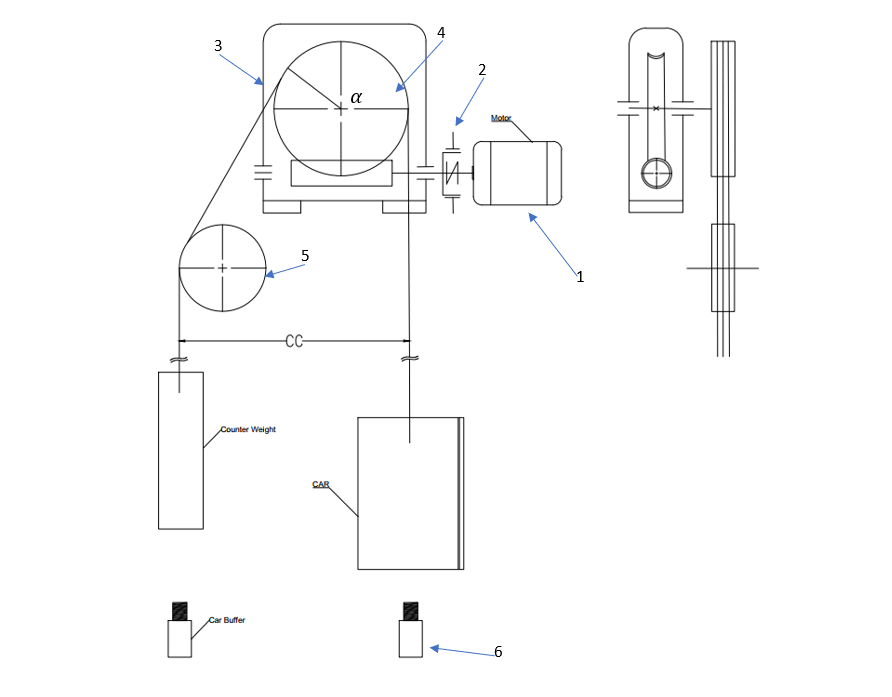
\includegraphics[width=21cm,height=16.8cm]{Image/so do co cau.png}}
    \caption[Dynamic diagram]{\bfseries \fontsize{12pt}{0pt}\selectfont Dynamic diagram}
    \label{figure1}
\end{figure}
\vspace{19.2cm}

\begin{table}[H]
    \centering
    
    \begin{tabular}{l l}
        \fontsize{12pt}{0pt}\selectfont 1.     \fontsize{12pt}{0pt}\selectfont Motor \\
        \fontsize{12pt}{0pt}\selectfont 2.   \fontsize{12pt}{0pt}\selectfont Flexible coupling\\
        \fontsize{12pt}{0pt}\selectfont 3.     \fontsize{12pt}{0pt}\selectfont Gearbox \\
        \fontsize{12pt}{0pt}\selectfont 4.     \fontsize{12pt}{0pt}\selectfont Pulley \\
        \fontsize{12pt}{0pt}\selectfont 5.     \fontsize{12pt}{0pt}\selectfont Orienting pulley \\

\end{tabular}
\end{table}

\section{Working principle of the elevators}

As the motor is activated by the users, its rotation is transmitted to the main sheave by the gear box. By the balanced-hoisting mechanism including the counterweight and the car, the gearbox therefore can easily move the car upward or downward. When the car shifts upward the counterweight is in downward motion and vice versa. The car stops at selected floor for carrying purposes.
To reduce the noise during operating time of the elevator, the gearbox should use the worm gear transmission. Worm gear transmission has the advantage of high gear ratio, small size and self braking.
Worm gear box can use the cylindrical worm or globoidal worm. Globoidal worm gear are widely used for elevator machines thanks to its smaller dimensions in comparison to the cylindrical type with the same power rating. 
The worm gear box can be manufactured with the worm placed above or below the worm gear. Traction sheave is attached directly to the worm. The wear of the traction sheave is usually high; therefore the sheave collar should be easily disassembled for replacement. The shaft of the worm is placed on the bearing. At an end of the worm which is opposite to the motor, a hand crank is attached so that we can control the machine manually. It is also removable.

\newpage